% Mutation-adequacy radar -- single-column.
%
% Design:
%   - hexagonal grid (concentric hexagons + 6 radial spokes)
%   - no vertex markers, no numerical value labels
%   - tools that cover >= 2 SUTs are drawn as filled polygons
%     (BioTest 6 axes, Pure-Random 6 axes, Jazzer triangle on
%      htsjdk-VCF + htsjdk-SAM, Atheris degenerate line on
%      vcfpy + biopython which are 180 deg apart)
%   - single-SUT tools (cargo-fuzz, libFuzzer, AFL++) are drawn
%     as a single coloured dot at the value position on their
%     applicable axis
%   - all polygon outlines are kept thin so the shaded areas
%     dominate over outline
%
% Width is sized for IEEEtran's single column (~88mm).

\begin{figure}[!t]
\centering
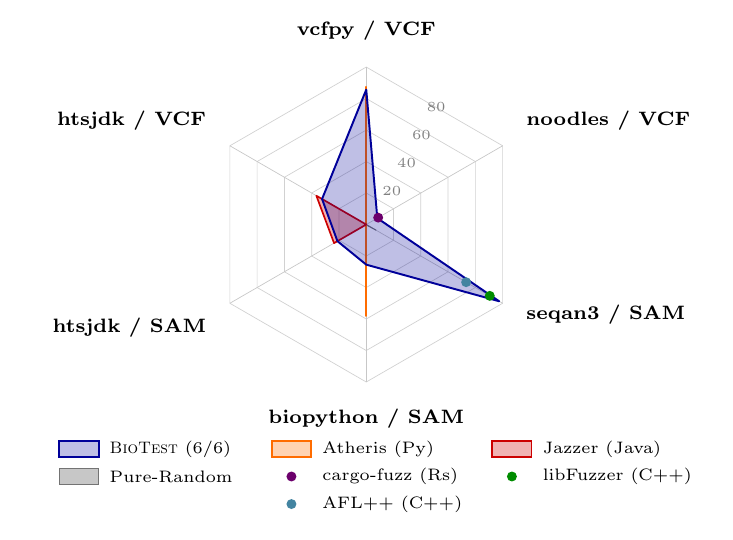
\begin{tikzpicture}

\colorlet{btblue}{blue!60!black}
\colorlet{atherisclr}{orange!85!red}
\colorlet{jazzerclr}{red!80!black}
\colorlet{cargoclr}{violet!85!black}
\colorlet{libfclr}{green!55!black}
\colorlet{aflclr}{cyan!60!black}
\colorlet{prclr}{black!55}

\pgfmathsetmacro{\R}{2.0}
\useasboundingbox (-4.3,-3.65) rectangle (4.3,2.50);

% ---- (1) hexagonal grid + spokes --------------------------------
\foreach \pct in {20,40,60,80,100}{%
  \draw[draw=black!18, line width=0.25pt, line join=round]
        (90:{\R*\pct/100}) -- (30:{\R*\pct/100})
     -- (-30:{\R*\pct/100}) -- (-90:{\R*\pct/100})
     -- (-150:{\R*\pct/100}) -- (150:{\R*\pct/100}) -- cycle;
}
\foreach \pct in {20,40,60,80}{%
  \node[font=\fontsize{5}{5.5}\selectfont, text=black!50,
        anchor=south west, inner sep=0.3pt]
        at (62:{\R*\pct/100}) {\pct};
}
\foreach \ang in {90,30,-30,-90,-150,150}{%
  \draw[draw=black!22, line width=0.25pt] (0,0) -- (\ang:\R);
}

% ---- (2) Pure-Random hexagonal floor (multi-SUT, shaded) -------
\filldraw[fill=prclr, fill opacity=0.40,
          draw=prclr, line width=0.35pt, line join=round]
   (90:{\R*0.0089}) -- (30:0) -- (-30:{\R*0.0719})
-- (-90:{\R*0.0024}) -- (-150:{\R*0.0120}) -- (150:0) -- cycle;

% ---- (3) Atheris (multi-SUT but two collinear axes; the polygon
%          is geometrically degenerate and renders as a thin
%          shaded line through the origin) -----------------------
\filldraw[fill=atherisclr, fill opacity=0.30,
          draw=atherisclr, line width=0.7pt, line join=round]
   (90:{\R*0.8737}) -- (30:0) -- (-30:0)
-- (-90:{\R*0.5800}) -- (-150:0) -- (150:0) -- cycle;

% ---- (4) Jazzer (multi-SUT, filled triangle in the left half) --
\filldraw[fill=jazzerclr, fill opacity=0.30,
          draw=jazzerclr, line width=0.6pt, line join=round]
   (90:0) -- (30:0) -- (-30:0)
-- (-90:0) -- (-150:{\R*0.2361}) -- (150:{\R*0.3659}) -- cycle;

% ---- (5) BioTest hexagon (top layer, dominant area) ------------
\filldraw[fill=btblue, fill opacity=0.25,
          draw=btblue, line width=0.7pt, line join=round]
   (90:{\R*0.8566}) -- (30:{\R*0.0810}) -- (-30:{\R*0.9744})
-- (-90:{\R*0.2548}) -- (-150:{\R*0.2114}) -- (150:{\R*0.3240})
-- cycle;

% ---- (6) Single-SUT tools as dots ------------------------------
\fill[cargoclr] (30:{\R*0.0874}) circle (1.8pt);
\fill[libfclr]  (-30:{\R*0.9057}) circle (1.8pt);
\fill[aflclr]   (-30:{\R*0.7322}) circle (1.8pt);

% ---- (7) per-axis SUT/format labels ----------------------------
\node[anchor=south, inner sep=1pt,
      font=\fontsize{7.5}{7.5}\selectfont\bfseries]
      at (90:{\R + 0.30}) {vcfpy / VCF};
\node[anchor=south west, inner sep=1pt,
      font=\fontsize{7.5}{7.5}\selectfont\bfseries]
      at (30:{\R + 0.30}) {noodles / VCF};
\node[anchor=west, inner sep=1pt,
      font=\fontsize{7.5}{7.5}\selectfont\bfseries]
      at (-30:{\R + 0.30}) {seqan3 / SAM};
\node[anchor=north, inner sep=1pt,
      font=\fontsize{7.5}{7.5}\selectfont\bfseries]
      at (-90:{\R + 0.30}) {biopython / SAM};
\node[anchor=north east, inner sep=1pt,
      font=\fontsize{7.5}{7.5}\selectfont\bfseries]
      at (-150:{\R + 0.30}) {htsjdk / SAM};
\node[anchor=south east, inner sep=1pt,
      font=\fontsize{7.5}{7.5}\selectfont\bfseries]
      at (150:{\R + 0.30}) {htsjdk / VCF};

% ---- (8) compact 3-row x 3-col legend below the radar ---------
\begin{scope}[shift={(0,-2.85)}]
  % Row 1: multi-SUT shaded tools
  \filldraw[fill=btblue, fill opacity=0.25,
            draw=btblue, line width=0.7pt]
            (-39mm,-1mm) rectangle (-34mm,1mm);
  \node[anchor=west, font=\fontsize{6.4}{7.2}\selectfont,
        inner sep=1pt] at (-33mm, 0)
        {\textsc{BioTest} (6/6)};

  \filldraw[fill=atherisclr, fill opacity=0.30,
            draw=atherisclr, line width=0.7pt]
            (-12mm,-1mm) rectangle (-7mm,1mm);
  \node[anchor=west, font=\fontsize{6.4}{7.2}\selectfont,
        inner sep=1pt] at (-6mm, 0)
        {Atheris (Py)};

  \filldraw[fill=jazzerclr, fill opacity=0.30,
            draw=jazzerclr, line width=0.6pt]
            (16mm,-1mm) rectangle (21mm,1mm);
  \node[anchor=west, font=\fontsize{6.4}{7.2}\selectfont,
        inner sep=1pt] at (22mm, 0)
        {Jazzer (Java)};
\end{scope}

\begin{scope}[shift={(0,-3.20)}]
  % Row 2: Pure-Random + first two single-SUT dots
  \filldraw[fill=prclr, fill opacity=0.40,
            draw=prclr, line width=0.35pt]
            (-39mm,-1mm) rectangle (-34mm,1mm);
  \node[anchor=west, font=\fontsize{6.4}{7.2}\selectfont,
        inner sep=1pt] at (-33mm, 0)
        {Pure-Random};

  \fill[cargoclr] (-9.5mm, 0) circle (1.8pt);
  \node[anchor=west, font=\fontsize{6.4}{7.2}\selectfont,
        inner sep=1pt] at (-6mm, 0)
        {cargo-fuzz (Rs)};

  \fill[libfclr] (18.5mm, 0) circle (1.8pt);
  \node[anchor=west, font=\fontsize{6.4}{7.2}\selectfont,
        inner sep=1pt] at (22mm, 0)
        {libFuzzer (C++)};
\end{scope}

\begin{scope}[shift={(0,-3.55)}]
  % Row 3: AFL++ alone
  \fill[aflclr] (-9.5mm, 0) circle (1.8pt);
  \node[anchor=west, font=\fontsize{6.4}{7.2}\selectfont,
        inner sep=1pt] at (-6mm, 0)
        {AFL++ (C++)};
\end{scope}

\end{tikzpicture}

\caption{Mutation kill rate per (SUT, format), means over $n$
replicates per tool ($n$ in \S\ref{sec:mutation-adequacy}).
Background: concentric hexagons at the $20/40/60/80/100\%$
levels with six radial axes. Tools spanning multiple SUTs (\biotest{},
Atheris, Jazzer, Pure-Random) are drawn as filled shaded
polygons; single-SUT tools (cargo-fuzz, libFuzzer, AFL++) are
drawn as a coloured dot at the value position on their
applicable axis.}
\label{fig:mutation-radar}
\end{figure}
